\documentclass[main]{subfiles}
\begin{document}
\chapter{8の字を走行}

これは講義資料「第2回 ロボットの動かし方と基本的な動作」内の課題です。

\section{課題概要}
ロボットを8の字を描くように走行させる。

なおこの実験ではセンサを利用しないため、周囲に何もない場所で開始する必要がある。

\section{解法}
\begin{figure}[H]
	\begin{minipage}{0.6\hsize}
		\setlength{\parindent}{1\Cwd}
		二つの円を描くにあたって
		円を切り替えるタイミングに注意する。
		先に反時計回りに上の円を描くのだが、
		原点のみで下の円の描画に切り替わるような判定をすると
		開始時に判定が行われ下の円しか描画されない。

		そこで、右図のように(1,0), (0,0), (-1,0)の3点に達した
		(正確には3点の半径1cm以内に入った)タイミングで
		命令が切り替わるように設計した。以下に命令列を書き下した。

		\begin{itemize}
			\item (0,1)に到達するまで上の円を描く
			\item (0,0)に到達するまで上の円を描く
			\item (0,-1)に到達するまで下の円を描く
			\item (0,0)に到達するまで下の円を描く
		\end{itemize}
	\end{minipage}
	\begin{minipage}{0.3\hsize}
		\begin{figure}[H]
			\centering
			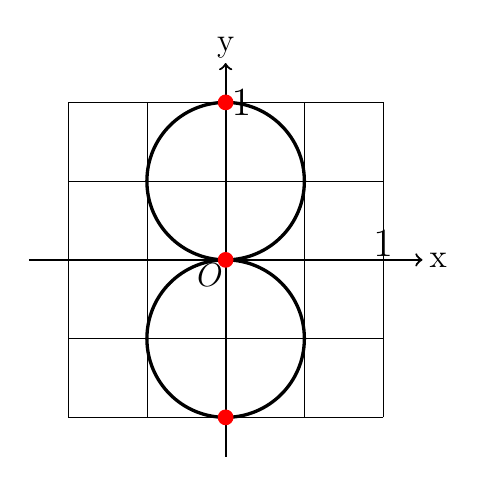
\begin{tikzpicture}[scale=1]
				\draw [ultra thin] (-2,-2) grid (2,2);
				\draw [thick,->] (-2.5,0) -- (2.5,0);
				\draw [thick,->] (0,-2.5) -- (0,2.5);
				\draw [very thick] (0,1) circle [x radius=1, y radius=1];
				\draw [very thick] (0,-1) circle [x radius=1, y radius=1];
				\node at (-0.2,-0.2) {\large $O$};
				\node at (2.7,0) {\large x};
				\node at (0,2.7) {\large y};
				\node at (0.2,2) {\Large $1$};
				\node at (2,0.2) {\Large $1$};

				\fill [red] (0,-2) circle [x radius=0.1, y radius=0.1];
				\fill [red] (0,0) circle [x radius=0.1, y radius=0.1];
				\fill [red] (0,2) circle [x radius=0.1, y radius=0.1];
			\end{tikzpicture}
			\caption{原点を出発して8の字を描くように進む}
		\end{figure}
	\end{minipage}
\end{figure}

\begin{figure}[H]
	\begin{minipage}{0.5\hsize}
		\setlength{\parindent}{1\Cwd}
		\section{結果}
		右図のように綺麗なオドメトリが計測できた。

		\section{考察}
		単純な課題ではあるが、開始時に上の円の描画命令を発行した後
		プログラムをスリープさせる等切り替えタイミングの解決法は複数考えられる。
	\end{minipage}
	\begin{minipage}{0.5\hsize}
		\begin{figure}[H]
			\centering
			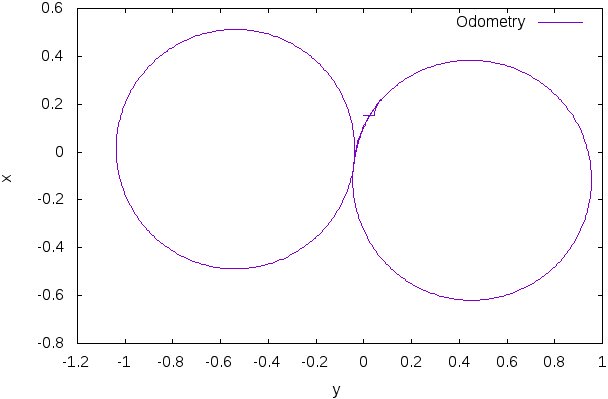
\includegraphics[width=8cm]{img/eight.png}
			\caption{8の字走行のオドメトリ}
		\end{figure}
	\end{minipage}
\end{figure}

\chapter{前方1m以内に障害物を見つけたら停止}

これは講義資料「第3回 測域センサの使い方」の課題です。

\section{課題概要}
\section{解法}

\section{結果}
\begin{figure}[H]
	\centering
	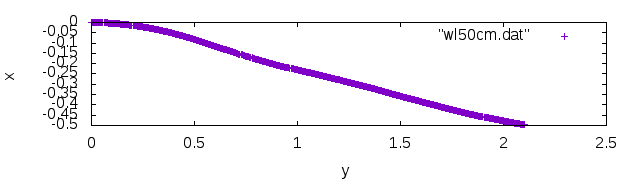
\includegraphics[width=15cm]{img/wl50cm.png}
\end{figure}
小刻みに調整が働いて壁と並行する線上を走行できていることがわかる。

\section{考察}


\end{document}
